\documentclass[a4paper,12pt]{article}

\usepackage[spanish,activeacute]{babel}
\usepackage{graphicx}

\title{Compromiso 1}
\author{Javier Falc\'on (2016-5265)}

\begin{document}

\maketitle
\section{Construcción de expresiones regulares.}

\begin{itemize}

\item[a.] Todas las cadenas de dígitos que representan números de matrículas válidos de PUCMM.

$\\digit = [0-9]$\\\\
$(\sim(0|1)digit^3)|digit^2-digit^4$\\

\item[b.] Todas las cadenas de dígitos que representan números telefónicos válidos.

$\\digit = [0-9]$\\\\
$+1-8(0|2|4)9-digit^7$

\item[c.] Todas las cadenas de alfanuméricas que representan direcciones de correo electrónico válidas.

$\\name = [a-zA-Z0-9\_-.]$ 
$\\domain = [a-zA-Z]$
$\\extension = [a-zA-Z]$

$name^+@domain^+.((extension^+).)^+extension^+$

\item[d.] Todas las cadenas alfanuméricas que representan direcciones web (URL) válidas.

$\\port = (ftp)|(http)|(https)|(file)$ 
$\\path = [a-zA-Z0-9]$

$port://[path^+(.(path^+)^+]?(/(path-)^+)^+$

\end{itemize}

\section{Construcción de autómatas}

\begin{figure}[h]
  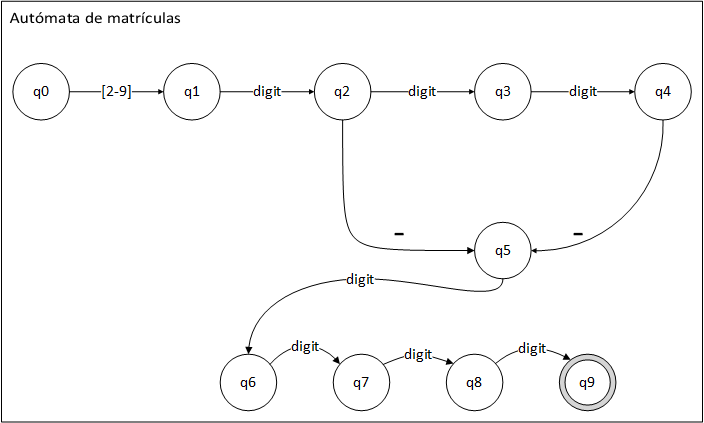
\includegraphics[width=\linewidth]{matricula.png}
  \caption{Autómata que representa el análisis léxico de las matrículas de PUCMM.}
  \label{fig:auto1}
\end{figure}


\begin{figure}[h]
  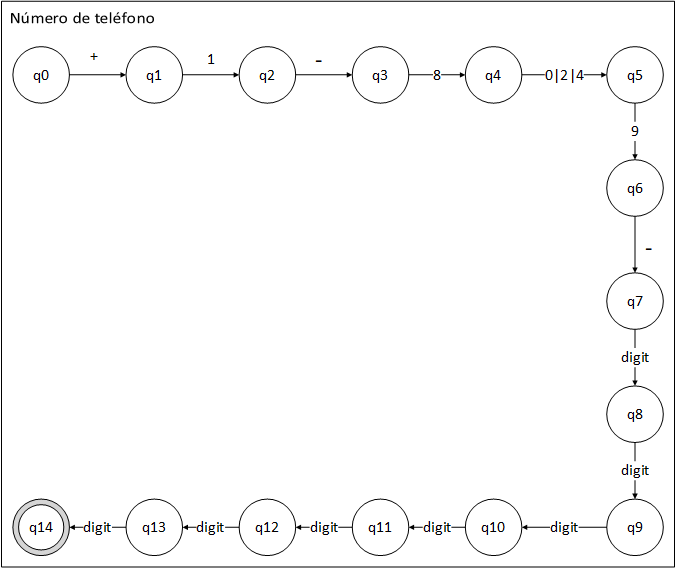
\includegraphics[width=\linewidth]{telefono.png}
  \caption{Autómata que representa el análisis léxico de los números de teléfono.}
  \label{fig:auto2}
\end{figure}

\begin{figure}[h]
  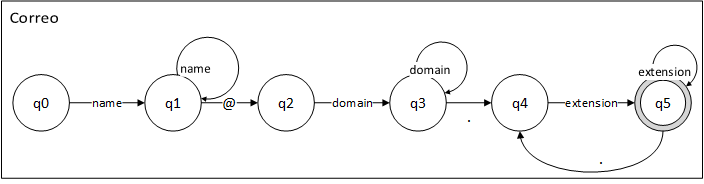
\includegraphics[width=\linewidth]{correo.png}
  \caption{Autómata que representa el análisis léxico de las direcciones de correo.}
  \label{fig:auto3}
\end{figure}

\begin{figure}[h]
  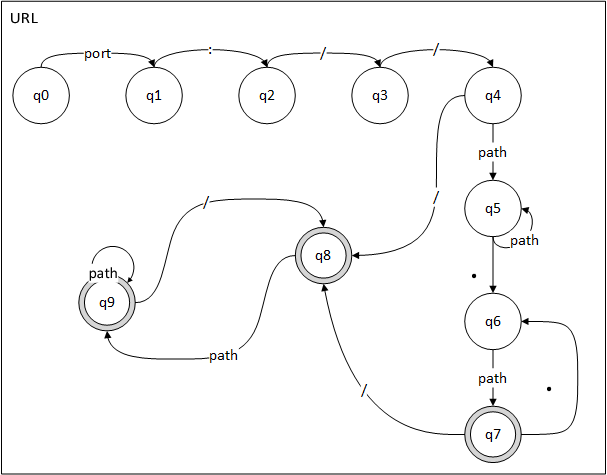
\includegraphics[width=\linewidth]{url.png}
  \caption{Autómata que representa el análisis léxico de las direcciones URL.}
  \label{fig:auto4}
\end{figure}

\end{document}